\chapter{MIPS}


\section{MIPS Instructions}

These are the three main instruction formats in the MIPS (Microprocessor without Interlocked Pipeline Stages) architecture: \bcode{R}, \bcode{I}, \bcode{J}

\subsection{R - Register Type}
R-type instructions are used for operations that involve only registers. They have three register operands and a function code to specify the operation.

\begin{center}
   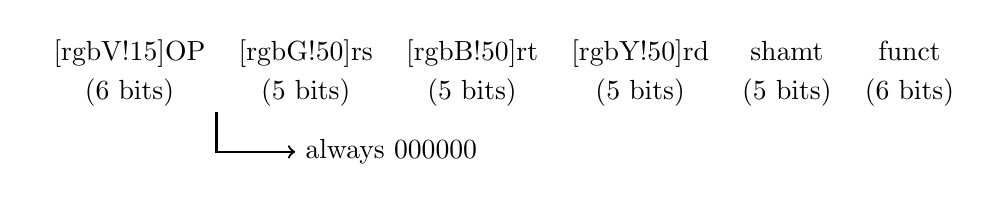
\begin{tikzpicture}
      \node (table) at (0,0) {
          \begin{tabular}{cccccc}
          \bcode[rgbV!15]{OP} & \bcode[rgbG!50]{rs} &
          \bcode[rgbB!50]{rt} & \bcode[rgbY!50]{rd} &
          \bcode{shamt} & \bcode{funct} \\[0.5ex]
          (6 bits) & (5 bits) & (5 bits) &
          (5 bits) & (5 bits) & (6 bits) \\
          \end{tabular}
      };
      \draw[thick, ->] (-3.65,-0.5) |- ++(1,-0.5) 
          node[right] {always {000000}};
   \end{tikzpicture}
\end{center}

\begin{tabular}{llll}
   \textbf{Example:}
   & \code{add \$t0, \$t1, \$t2}
   & $\to$ \, (Addition) \,\, \code{\$t0 = \$t1 + \$t} \\
   & \code{sll \$t0, \$t1, 2}
   & $\to$ \, (Shift Left) \,\, \code{\$t0 = \$t1 << 2}
\end{tabular}

\subsection{I - Immediate Type}
I-type instructions are used for operations that involve an immediate value (a constant) and registers. They have two register operands and a 16-bit immediate value.

\begin{center}
   \begin{tabular}{cccccc}
      \bcode[rgbV!15]{OP} &
      \bcode[rgbG!50]{rs} &
      \bcode[rgbB!50]{rt} &
      \bcode[rgbY!50]{IMM} \\[0.5ex]
      (6 bits) & (5 bits) & (5 bits) & (16 bits) \\
   \end{tabular}
\end{center}


\begin{tabular}{llll}
   \textbf{Example:}
   & \code{lw \$t0, 4(\$t1)} 
   & $\to$ \, Load word from memory at address 
   \code{(\$t1+4)} into \code{\$t0}\\
\end{tabular}

\subsection{J - Jump Type}
J-type instructions are used for jump operations, which change the program counter to a new address. They have a 26-bit target address.

\begin{center}
   \begin{tabular}{cccccc}
      \bcode[rgbV!15]{OP} & \bcode[rgbY!50]{Pseudo Address} \\[0.5ex]
      (6 bits) & (26 bits) \\
   \end{tabular}
\end{center}

\begin{tabular}{llll}
   \textbf{Example:}
   & \code{j TARGET}
   & Jump to the instruction at address TARGET\\
   & \code{jal FUNCTION}
   & Jump to FUNCTION and save return address in \code{\$ra}\\
\end{tabular}


\pagebreak
\section{Common MIPS Instruction Set}

\subsection{Arithmetic Instructions}
\begin{multicols}{3}
   \begin{itemize}[parsep=0pt]
      \item \texttt{add} - Add two registers
      \item \texttt{addi} - Add reg and immediate
      \item \texttt{addu} - unsinged
      \item \texttt{sub} - Subtract two registers
      \item \texttt{subi} - Sub reg and immediate
      \item \texttt{subu} - sub unsigned
      \item \texttt{mul} - Multiply two registers
      \item \texttt{div} - Divide two registers
   \end{itemize}
\end{multicols}

\subsection{Logical Instructions}
\begin{multicols}{3}
   \begin{itemize}[parsep=0pt]
      \item \texttt{and} - Bitwise AND
      \item \texttt{or} - Bitwise OR
      \item \texttt{xor} - Bitwise XOR
      \item \texttt{nor} - Bitwise NOR
      \item \texttt{not}- Bitwise Not
   \end{itemize}
\end{multicols}

\subsection{Shift Instructions}
\begin{multicols}{3}
   \begin{itemize}[parsep=0pt]
      \item \texttt{sll} - Shift Left Logical
      \item \texttt{srl} - Shift Right Logical
      \item \texttt{sra} - Shift Right Arithmetic
   \end{itemize}
\end{multicols}

\subsection{Memory Access Instructions}
\begin{multicols}{2}
   \begin{itemize}[parsep=0pt]
      \item \texttt{lw} - Load Word (from memory to a register)
      \item \texttt{sw} - Store Word (from a register to memory)
      \item \texttt{lb} - Load Byte (from memory to a register)
      \item \texttt{sb} - Store Byte (from a register to memory)
   \end{itemize}
\end{multicols}

\subsection{Control Flow Instructions}
\begin{multicols}{2}
   \begin{itemize}[parsep=0pt]
      \item \texttt{beq} - Branch if Equal
      \item \texttt{bne} - Branch if Not Equal
      \item \texttt{j} - Jump to a specified address
      \item \texttt{jal} - Jump and Link (used for function calls)
      \item \texttt{jr} - Jump Register (used for returning from a function)
   \end{itemize}
\end{multicols}

\section{MIPS Registers}

\begin{tabularx}{\textwidth}{|l|c|l|X|c|}
      \hline
      \textbf{Register} & \textbf{\#Reg no.} & \textbf{Name} & \textbf{Usage} & \textbf{Preserved across calls?} \\
      \hline
      \texttt{\$zero}  & 0 & Zero Register   & Always holds \texttt{0} & Yes \\
      \texttt{\$at}    & 1 & Assembler Temp  & Reserved for assembler (pseudo-instructions) & No \\
      \texttt{\$v0-\$v1} & 2-3 & Return Values  & Used for function return values & No \\
      \texttt{\$a0-\$a3} & 4-7 & Arguments      & Used to pass function arguments & No \\
      \bcode[rgbB!50]{\$t0-\$t7} & \bcode[rgbY!50]{8-15} & Temporary      & Used for temporary values & No \\
      \bcode[rgbB!50]{\$s0-\$s7} & \bcode[rgbY!50]{16-23} & Saved Registers & Used for saved values, preserved across calls & Yes \\
      \bcode[rgbB!50]{\$t8-\$t9} & \bcode[rgbY!50]{24-25} & Temporary      & Additional temporary registers & No \\
      \texttt{\$k0-\$k1} & 26-27 & Kernel Reserved & Used by the OS kernel & N/A \\
      \texttt{\$gp}    & 28 & Global Pointer  & Points to global variables & Yes \\
      \texttt{\$sp}    & 29 & Stack Pointer   & Points to the top of the stack & Yes \\
      \texttt{\$fp}    & 30 & Frame Pointer   & Used for function stack frames & Yes \\
      \texttt{\$ra}    & 31 & Return Address  & Stores return address for function calls & No \\
      \hline
\end{tabularx}

\red{\ding{74}}
\code{Memory Address = 4 * Offset + Base Address}

\pagebreak
\section{MIPS Problems}

\textbf{\textit{\#Question:}}
Let, A = 5, B = 5, and C = 0.
If A is not equal to B, subtract B from A and store the result in C.
Otherwise, add A and B and store the result in C.
Now write the MIPS instructions for the given problem.


\textbf{\textit{Solution}:}
\begin{multicols}{2}
   \noindent
   \raggedcolumns
   
\begin{verbatim}
   # Load values into registers
   li $t0, 5       # A = 5 ($t0)
   li $t1, 5       # B = 5 ($t1)
   li $t2, 0       # C = 0 ($t2)

   beq $t0, $t1, SUM 

   sub $t2, $t0, $t1
   j END

   SUM:
      add $t2, $t0, $t1

   END:
      jr $ra
\end{verbatim}
  
  \columnbreak

\begin{verbatim}
   int a = 5;
   int b = 5;
   int c = 0;

   if (a != b) {
      c = a - b;
   } else {
      c = a + b;
   }
\end{verbatim}
\end{multicols}




\textbf{\textit{\#Question:}}
Let, i = 0, sum = 0, and limit = 5.
Using a while loop, keep adding i to sum and incrementing i until i is no longer less than limit.
Now write the MIPS instructions for this problem.

\textbf{\textit{Solution}:}
\begin{multicols}{2}
\noindent
\raggedcolumns
   
\begin{verbatim}
   .data

   .text
   .globl main
   main:
       li   $t0, 0
       li   $t1, 0
       li   $t2, 5
   
   loop:
       beq  $t0, $t2, end
       add  $t1, $t1, $t0
       addi $t0, $t0, 1
       j    loop
   
   end:
       jr   $ra
\end{verbatim}
\columnbreak

\begin{verbatim}
   int i = 0;        => $t0
   int sum = 0;      => $t1
   int limit = 5;    => $t2

   while (i < limit) 
      sum = sum + i;
      i = i + 1;
   }
\end{verbatim}
\end{multicols}


\pagebreak
\textbf{\textit{Question:}}
Instruction and Opcode/Function: \texttt{lw 100011}, \texttt{sub 101011}, \texttt{sub 100010}, \texttt{add 100000}. Analyze the following high level statement according to MIPS instruction format and write the MIPS machine code.\\\code{A[40] = B - A[60]};

\textbf{\textit{Solution:}}
\begin{verbatim}
   lw  $t0, 240($s0)           # Load A[60] into $t0
   sub $t1, $s1, $t0           # Subtract B from A[60]
   sw  $t1, 160($s0)           # Store result into A[40]
\end{verbatim}